\documentclass[11pt]{article}

\usepackage{comment} % enables the use of multi-line comments (\ifx \fi) 
\usepackage[a4paper,margin=1cm]{geometry}
\usepackage[utf8]{inputenc}
\usepackage[ngerman]{isodate}
\usepackage{gensymb}
\usepackage{graphicx}
\usepackage{booktabs}% http://ctan.org/pkg/booktabs
\usepackage{tabularx}
\usepackage{ltablex} % Longtables with tabularx
\usepackage[x11names]{xcolor}
\usepackage{amsmath}
\usepackage{amssymb}
\usepackage{amsthm}
\usepackage{array}
\usepackage{wrapfig}
\usepackage{subcaption}
\usepackage{csquotes}
\usepackage{lscape}
\usepackage{geometry}
\usepackage{multicol}
\usepackage{bm}
\usepackage{enumitem}
\usepackage{hyperref}
\usepackage{mdframed}
\usepackage{scalerel}
\usepackage{stackengine}
\usepackage{mathtools}
\usepackage{pdfpages}

% Code highlighting
\usepackage{minted}
\surroundwithmdframed{minted}

% Be able to caption equations and float them in place
\usepackage{float}

\newmdtheoremenv{theorem}{Theorem}
\geometry{a4paper, margin=2.4cm}
\newtheorem*{remark}{Remark}

\newcommand\equalhat{\mathrel{\stackon[1.5pt]{=}{\stretchto{\scalerel*[\widthof{=}]{\wedge}{\rule{1ex}{3ex}}}{0.5ex}}}}
\newcommand\defeq{\mathrel{\overset{\makebox[0pt]{\mbox{\normalfont\tiny def}}}{=}}}
\newcolumntype{C}{>{\centering\arraybackslash}X}

\DeclarePairedDelimiter\abs{\lvert}{\rvert}
\DeclarePairedDelimiter\norm{\lVert}{\rVert}

\setcounter{tocdepth}{3}
\setcounter{secnumdepth}{3}

\graphicspath{{./img/}}

\begin{document}
	
\title{Analysis of Text Data FS20}
\author{Pascal Baumann\\pascal.baumann@stud.hslu.ch}
\maketitle



For errors or improvement raise an issue or make a pull request on the \href{https://github.com/KilnOfTheSecondFlame/mse_summaries}{github repository}.

\tableofcontents
\newpage

\section{Introduction}
Text analysis consist of a series of operations completed by one or more pieces of software on a sample of written human language, with the goal of extracting useful information.

Applications of text analysis include:
\begin{itemize}[noitemsep]
	\item Analysis
	\begin{itemize}
		\item spell checkers
		\item keyword extraction
		\item authorship attribution
		\item document retrieval
		\item text classification
		\item text mining
		\item sentiment analysis
		\item content-based recommendation
	\end{itemize}
	\item Text Analysis and Generation
	\begin{itemize}
		\item machine translation
		\item automatic question answering
		\item automatic summarisation
	\end{itemize}
	\item Text Generation
	\begin{itemize}
		\item database report generation
		\item weather forecast generation
	\end{itemize}
	\item Analysis, Generation and Interaction
	\begin{itemize}
		\item dialogue systems
		\item assistive technology for teaching or writing
	\end{itemize}
\end{itemize}

Analysis of Text Data lies at the intersection of Machine Learning, Computational Linguistics and Human-Computer Interaction. Artificial Intelligence is applied to human language, while human speech data is a related problem which makes use of different technologies, like signal processing.

\subsection{Basic Concepts in NLP}
Machine Learning is a powerful tool in NLP, thus the same vocabulary is used. For Text Analysis supervised learning is used mostly, where the labelled data is classified by human experts and is called the reference or ground truth.

Significance addresses the key question if the difference between the two systems is really due to the fact that one is better than the other or if it can be explained by randomness. This is easier to compute when cross-validation is used, and paired $t$-tests can be used to compare two systems. Performance scores vary depending on the data set it is difficult to predict actual performance on a data set of a different
nature than the test set, this is called the problem of portability.

\subsection{Key Jargon from Linguistic}
\begin{itemize}
	\item letter
	\item syllable
	\item morpheme: a meaningful morphological unit of a language that cannot be further divided
	\item word
	\item phrase: a group of words standing together as a conceptual unit
	\item clause: a group of words in a sentence that contains a subject and a subject
	\item sentence:
	\begin{itemize}
		\item simple sentence: one independent clause
		\item compound sentence: at least two independent clauses
		\item complex sentence: at least one independent clause and one or more dependent clauses
	\end{itemize}
	\item text
	\item corpus: collection of text, pl. corpora
	\item utterance: an uninterrupted chain of spoken or written language
	\item lexeme: basic abstract unit of meaning that roughly corresponds to a set of forms taken by a single root word - for example run, runs, ran and running are forms of the same lexeme
	\item lemma:  one form chosen by convention as the canonical form of a lexeme - go, goes, went, gone, going for the lexeme \emph{go}
\end{itemize}

\subsection{Utterance Decoding}
Decode its propositional content or logical form first and then combine them. Draw inference to solve ambiguities, guess what is left unsaid and, in general, maximise the likelihood given the context.

\subsection{Lexical Analysis}
The goal of lexical analysis is to understand word forms.
\begin{enumerate}
	\item tokenisation: breaking a text into word tokens
	\item lemmatisation: finding the base form of each word token or lemma
	\item Part of Speech tagging: finding the part of speech each word token corresponds to
	\item Named Entity Recognition:  identification of proper nouns of people, places, organizations
\end{enumerate}

\subsection{Syntactic Analysis}
\begin{itemize}
	\item sentence segmentation or splitting
	\item identifying phrases or chunking
	\item figuring out logical functions
	\item building parse trees or parsing
\end{itemize}

\subsubsection{Constituency Parsing}
With syntactic parsing the connection between words can be understood. Constituency parsing breaks a sentence into its basic building blocks.

\begin{center}
	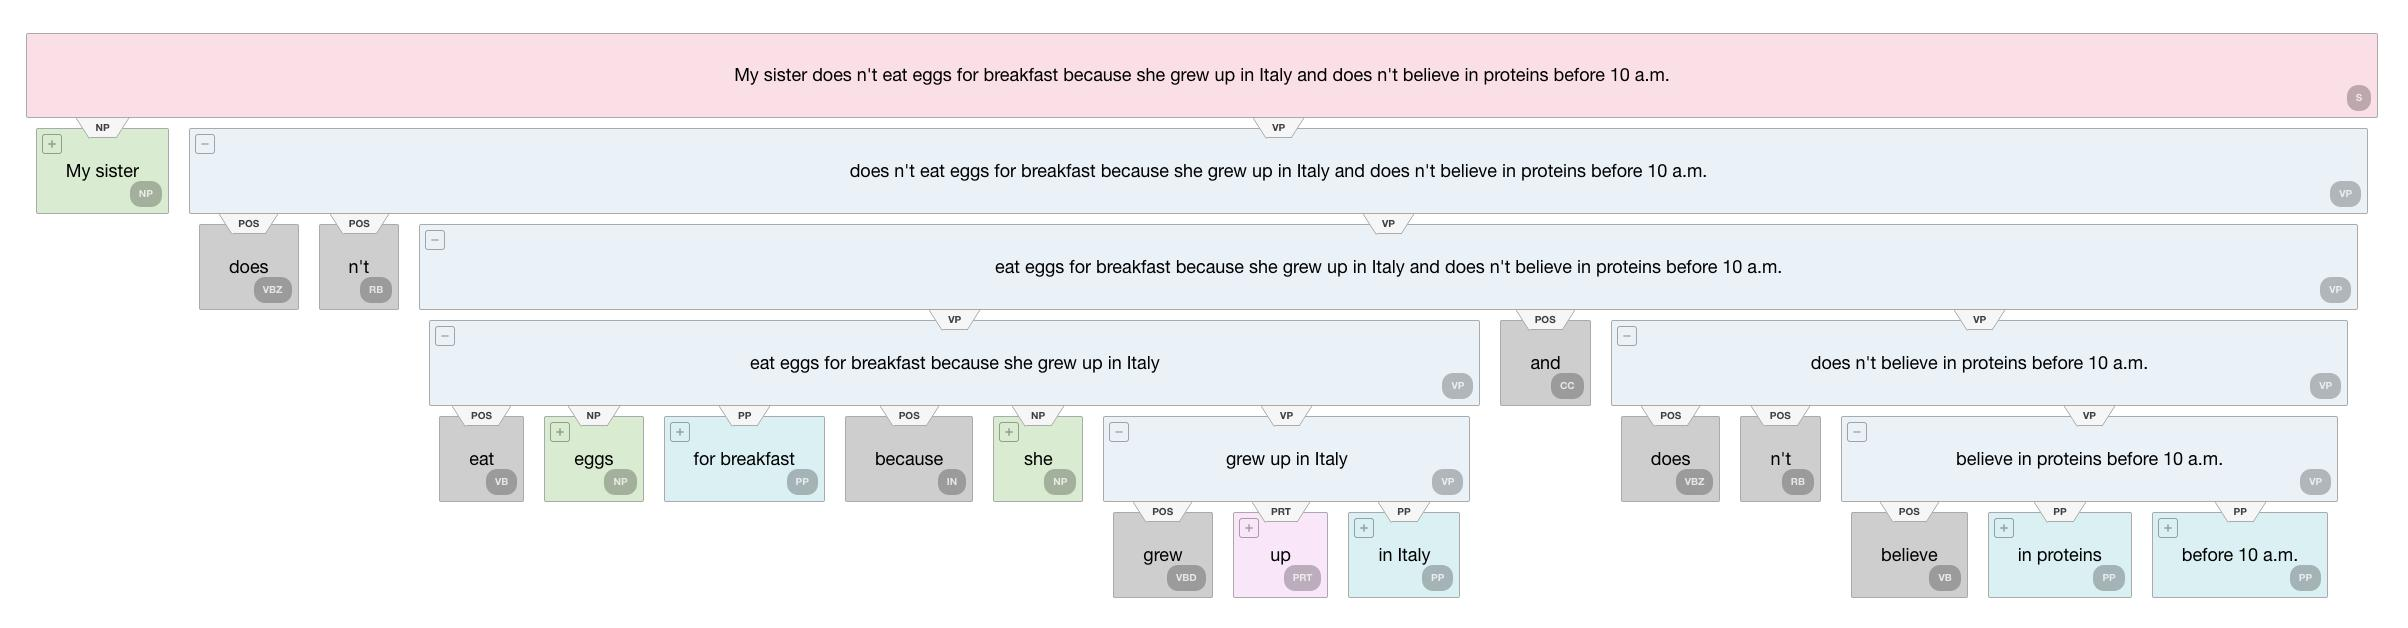
\includegraphics[width=\linewidth]{img/parse_tree_syntactic_parsing}
\end{center}

\subsubsection{Dependency Parsing}
Dependency Parsing helps in understanding what depends on what. The assumption is that the sentence is centred around the verb and what comes first in a sentence is more important than any information that comes after. So anything of the sentence depends on that word or some lower-level information.

\begin{center}
	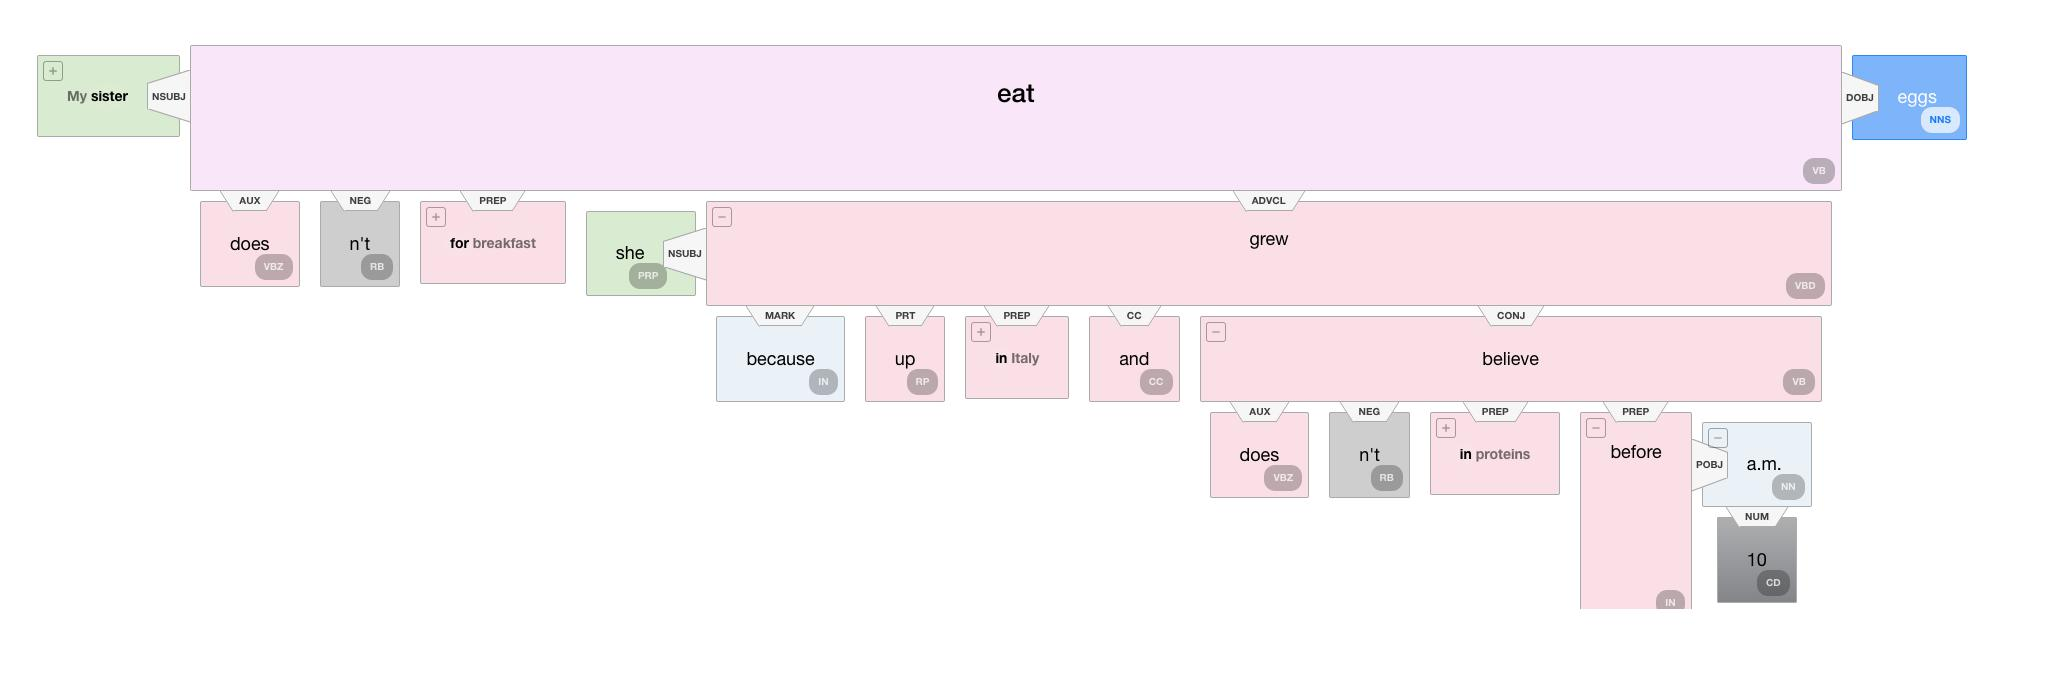
\includegraphics[width=\linewidth]{img/parse_tree_dependency_parsing}
\end{center}

\subsection{Understanding Meaning}
\subsubsection{Semantic Analysis}
\begin{itemize}
	\item word-level
	\begin{itemize}
		\item word sense disambiguation
		\item co-occurrence analysis
	\end{itemize}
	\item sentence-level or text-level
	\begin{itemize}
		\item semantic role labelling
		\item co-reference resolution
	\end{itemize}
\end{itemize}

\subsubsection{Discourse Analysis}
\begin{itemize}
	\item topics
	\item sentiments
	\item speech or dialogue acts
	\item argumentative structures
\end{itemize}

\subsection{Data for Text Analysis}
Text analysis using machine learning requires large amounts of training data and finding suitable data is often a bottleneck due to expense or limited rights. An annotated corpus typically contains a selection of texts based on explicit criteria, metadata like author, date, source, title, sectioning, and annotations in a more or less standardises format.

\subsection{Preprocessing}
Most text processing tasks begin with a set of standard preprocessing steps
\begin{itemize}
	\item Tokenisation: segmentation into tokens
	\item Token normalisation
	\item Segmentation into sentences
	\begin{center}
		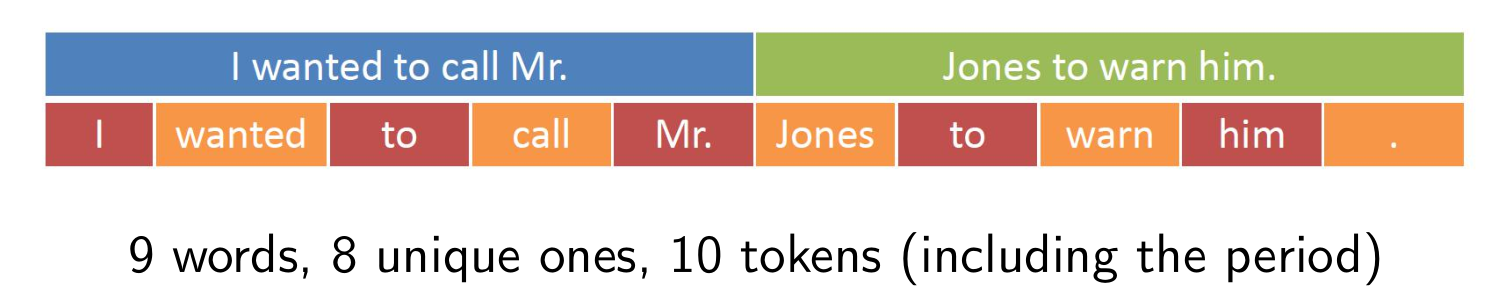
\includegraphics[width=0.8\linewidth]{img/sentence_segmentation}
	\end{center}
	\item There are about 170'000 unique words in the English language at the moment
\end{itemize}

\subsubsection{Tokens and Types}
Tokens are the words on the page, while the type is the word forms. Counting the types requires lemmatisation, which is finding the lemma or base form for each word.

\subsubsection{Tokenisation and Normalisation}
Not as straightforward as one may think
\begin{itemize}
	\item punctuation
	\begin{itemize}
		\item periods and commas appear within words or abbreviations
		\item special tokens in mail addresses or tweets
		\item apostrophes
	\end{itemize}
	\item capital letters
	\item compound words
	\begin{itemize}
		\item problem complicated without dashes
		\item German words
		\item proper names
	\end{itemize}
\end{itemize}

\subsubsection{Sentence Segmentation}
Can be easier or more difficult depending on the source text formatting. If no particular information is available from the layout, punctuations and casing can be used. While question and exclamation marks are quite reliable indicator of sentences periods are not. A good approach is to try to combine Tokenisation and Sentence Splitting, focusing on full stops.

\section{Text Classification}
The goal of text classification is to assign text documents to one or more categories. There is a predefined set of classes, in which previously unseen documents are assigned to. If there are only two classes this is a binary classification problem.

To tackle this problem there are different strategies: (a) have hard-coded rules carefully crafted by an expert on the basis on combinations of words or other features, (b) through supervised machine learning with understanding building on semantic representation of texts and labels or (c) supervised machine learning without understanding where word-based features are derived from text and the relationship between features and labels from the training texts.

Stopwords are words like conjunctions or preposition, which may not have meaning given the task at hand.

\subsection{Formalising Text Classification}

\begin{itemize}[label=]
	\item Input
	\begin{itemize}
		\item a set of documents $D$
		\item a fixed set $N$ of classes $C$
		\item a training set of $M$ hand-labelled documents $(d_1 C_1),(d_2 C_2), \dots (d_M C_M)$
	\end{itemize}
	\item Output
	\begin{itemize}
		\item a mapping $D\rightarrow C$ that associates a predicted class $c\in C$ to each document $d\in D$
	\end{itemize}
\end{itemize}

\subsection{Naïve Bayes Classifier}
For a document $d$ and a class $c$

\begin{equation*}
	P(c|d) = \frac{P(d|c)P(c)}{P(d)}
\end{equation*}

\noindent
Maximum A Posteriori (MAP) classifier:
\begin{equation*}
	c_{\text{MAP}} = \underset{c\in C}{\text{argmax}} \frac{P(d|c) P(c)}{P(d)} = \underset{c\in C}{\text{argmax}} P(d|c) P(c)
\end{equation*}

Dropping the denominator does not change $c_{\text{MAP}}$ because $P(d)$ has no effect on argmax. In practice, the evidence a machine can observe is not the human-readable document $d$, but a number of features $x_1,\dots,x_N$ obtained based on $d$ and a MAP-classifier
\begin{equation*}
	c_MAP = \underset{c\in C}{\text{argmax}} P(x_1, x_2, \dots , x_N | c) P(c)
\end{equation*}

\noindent
Given a vocabulary of V words a feature can be if a word appears in a document $d$ or how often it appears
\begin{itemize}
	\item \textbf{Bernoulli Model} represent $d$ as $(e_1, \dots, e_V)$ where $e_i =1$ if the word $i$ is in $d$ and $e_i = 0$ otherwise
	\item \textbf{Multinomial Model} represent $d$ as $f_1, \dots, f_V)$ where $f_i$ is the number of occurrences of word $i$ in $d$
\end{itemize}

The Naïve Bayes independence assumption is that given a class $c$ the \textbf{features are independent}
\begin{equation*}
	P(x_1, x_2, \dots , x_N | c) = P(x_1|c)\cdot P(x_2|c) \cdots P(x_N|c) = \prod_{k=1}^{n}P(x_k|c)
\end{equation*}

$P(c)$ and $P(x_k|c)$ need to be computed, $P(c)$ can be estimated based on the frequency of each class in the training data, and $P(x_k|c)$ depends on the chosen feature representation.

In the so called Bag-Of-Word Model $x_k$ is the feature representation of the words in the documents. The position of the individual words can usually be ignored.

\subsection{Multinomial Naïve Bayes}
Represent every token in $d$ as a feature vector $x_i = f_i$ , where $f_i$ is the number of occurrences of token $i$ in $d$. Then $P(x_i|c)$ can be estimated as $\frac{\text{number of occurrences of token }i\text{ in }c}{\text{total number of tokens in }c}$. For simplicity $P(w|c)$ can be written to refer to the probability of finding token $w$ in class $c$.

\begin{enumerate}
	\item Normalise the training data (remove stop words, remove punctuation, set all characters to lowercase)
	\item Assemble vocabulary (list of unique meaningful words)
	\item Count the number of occurrences of each word in each class and divide by the total number of words in each class
\end{enumerate}

\subsection{Practical Complications}
If a word $w$ from the vocabulary (which contains $V$ tokens) is never in class $c$ in the training data, we will estimate $P(w|c) = 0$, which causes $c_{\text{corpus}}=\underset{c\in C}{\text{argmax}}P(c)\prod_{k=1}^{N}P(x_k|c)=0$.

\begin{remark}
	Zero probabilities cannot be conditioned away, no matter the other evidence!\\ - Dan Jurafsky
\end{remark}

The typical solution to this is to do Laplace Smoothing like this
\begin{equation*}
	P(w|c)\text{ can be estimated as }\frac{\text{number of occurrences of token $w$ in class } c + 1}{\text{total number of tokens in class } c+V}
\end{equation*}
This prevents probabilities of zero to occur.

\subsection{Metrics}
\begin{itemize}[leftmargin=*, labelindent=3cm, labelsep=1cm]
	\item[True Positive] Sample $c$ classified correctly
	\item[False Positive] Non-$c$ sample incorrectly classified as $c$
	\item[True Negative] Non-$c$ sample classified correctly
	\item[False Negative] Sample $c$ classified incorrectly as non-$c$
\end{itemize}

\begin{tabularx}{\linewidth}{rX}
	Accuracy & $ \frac{\sum TP}{\sum \text{all elements}} $ \\
	Precision & $\frac{TP}{TP + FP}$\\
	Recall & $ \frac{TP}{TP + FN} $\\
\end{tabularx}

\section{Sentiment Analysis}
Sentiment analysis tries to understand the emotional state of the author of a text, and is also called opinion mining but can be extremely hard. In principle text classification and sentiment analysis are very different, but there are some striking similarities as the text can reflect a positive or a negative emotional state which can be utilised.

\subsection{Framing Sentiment Analysis}
Sentiment analysis is commonly framed as \textbf{attitude detection}
\begin{itemize}
	\item \emph{Attitude} is an enduring disposition toward someone or something with an emotional connotation
	\item The attitude can be broken down in quintuplets
	\begin{enumerate}
		\item opinion holder
		\item target entity
		\item aspect: specific feature of the target that the opinion is about
		\item type: most commonly {\color{green} positive}, {\color{red} negative}, {\color{gray} neutral} and with an indication of strength
		\item time when this opinion was expressed
	\end{enumerate}
	\item knowing the opinion without knowing the opinion target is of limited use
\end{itemize}

\subsection{Tokenisation Challenges}
\begin{itemize}
	\item Isolating emoticons
	\item Respecting domain-specific markup like \mintinline{html}{<strong>really bad idea</strong>}
	\item Capturing masked curses
	\item Selective true-casing
	\item Normalised lengthening, as "YAAAAAAY" is equivalent to "YAY" no matter how it is written
	\item Capturing important multi-word expressions and idioms
\end{itemize}

\subsubsection{Dealing With Negations}
A simple effective workaround by Das and Chen is to prepend \texttt{NOT\_} to every word between a negation and a clause-level punctuation mark.

\subsubsection{More Complications}
\begin{itemize}
	\item Modal adverbs like \emph{quite possibly, totally}
	\item Thwarted expectations "\emph{It was hailed as brilliant, unprecedented artistic achievement worthy of multiple Oscars}"
	\item Non-literal language "\emph{Like 50 hours long}"
\end{itemize}

\subsection{Various Degrees of Complexity}
In principle, all quintuplets in a document should be discovered, which would allow to represent unstructured information in a structured form. However, this is extremely hard to do. In practice, simplified forms of sentiment analysis are typically solved
\begin{itemize}
	\item Document-level sentiment classification
	\item Sentence-level sentiment classification
	\item Aspect-level sentiment classification
\end{itemize}
Though simplified, these forms of sentiment analysis are still hard to do with subtlety and sarcasm complicating the task.

\subsubsection{Document-level Sentiment Classification}
Does the document reflect an overall {\color{green} positive} or {\color{red} negative} view? The approach is the same as for text classification
\begin{enumerate}
	\item tokenisation
	\item feature extraction
	\item classification (Naïve Bayes, MaxEnt, SVM)
	\item Two or Three classes \{ {\color{green} positive} $\vert$ {\color{red} negative} $\vert$ ({\color{gray} neutral}) \}
\end{enumerate}

\subsection{Generative versus Discriminative Models}
In Naïve Bayes, for a document $d$ and each class $c$:
\begin{itemize}
	\item Estimate $P(d|c)$ and $P(c)$ directly from the training data
	\item Learn a model of $P(d\cap c) = P(d|c)\cdot P(c)$
	\item Use Bayes' rule to compute $P(c|d)=\dfrac{P(d|c)\cdot P(c)}{P(d)}$
	\item Pick the class that maximises $P(c|d)$ over all classes
\end{itemize}
This is called a \textbf{generative model}: Which class $c$ is most likely to have generated my test sample $d$, given the $P(d\cap c)$ that was estimated.

\noindent
The alternative is a \textbf{discriminative model} that models $P(c|d)$ directly.

\subsection{Discriminative Model: Maximum Entropy}
Entropy in information theory refers to a measure of the information content, where highly probable events carry very little information and if all events are equally likely there is maximum entropy. A prediction on which one will occur is impossible and when a event occurs there is a lot of learning.
\begin{itemize}
	\item Suppose movie reviews get classified into \{ {\color{Green3} positive} $\vert$ {\color{Firebrick3} negative} $\vert$ ({\color{gray} neutral}) \}
	\item In the training corpus 90\% of the sample containing the word \texttt{love} are tagged as {\color{Green3} positive}
	\item Let it further be that a test sample with the word \texttt{love} is 90\% likely to be positive and equally likely to be either {\color{Firebrick3} negative} (10\%) or {\color{gray} neutral} (10\%)
	\item All other things unknown are assumed to be equally likely (maximum entropy)
\end{itemize}
Unlike in text classification, topic words are not as important as \textbf{sentiment words} that carry an emotional charge, but the mapping between emotional states and the written word can be exceedingly subtle
\begin{itemize}[label=-]
	\item {\color{Green3} good}, {\color{Green3} splendid}, {\color{Green3} nice}
	\item {\color{Firebrick3} bad}, {\color{Firebrick3} racist}, {\color{Firebrick3} dismal}
\end{itemize}

\subsection{Unsupervised Sentiment Classification}
\begin{enumerate}
	\item Use a Part-Of-Speech tagger to identify phrases with adjectives and adverbs
	\item Estimate the semantic orientation
	\item Classify based on the average semantic orientation
\end{enumerate}
Semantic orientation is computed based on Pointwise Mutual Informaiton (PMI)
\begin{equation*}
\text{PMI} (w_1,w_2) = \log_2 \left( \frac{P(w_1,w_2)}{P(w_1)P(w_2)} \right) = \log_2 \left( \frac{P(w_1 | w_2)}{P(w_1)} \right) = \log_2 \left( \frac{P(w_2 | w_1)}{P(w2)} \right)
\end{equation*}
PMI is computed using approximate probabilities with normalised word counts in a corpus. Or the web can be used as a corpus using the number of hits from a search engine when $w_1$ and $w_2$ are searched. Following Barrière (2016) the number of hits of \texttt{the, a, of} are used, which results in a total of $2.527\cdot 10^10$ hits.
\subsubsection{Example PMI of Academy and Awards}
\begin{itemize}
	\item $w_1 = \text{\texttt{Academy}}$, $w_2 = \text{\texttt{Awards}}$
	\item $P(w_1,w_2) \propto \text{\#\texttt{Academy} AND \texttt{Awards}} \approx 1.01\cdot 10^9\text{hits}$
	\item $P(w_1) \propto \text{\#\texttt{Academy}} \approx 1.94\cdot 10^9 \text{hits}$
	\item $P(w_2) \propto\text{\#\texttt{Awards}} \approx 5.57\cdot 10^9\text{hits} $
	\item $\text{PMI}(w_1,w_2) \approx \log_2\left( \frac{1.01\cdot 10^9\cdot2.527\cdot 10^10}{1.94\cdot 10^9\cdot 5.57\cdot 10^9} \right)\approx 1.24 $
\end{itemize}
Two words with high PMI are very likely to occur jointly, while two words with low PMI are very likely to occur separately. PMI can also be used to compute Semantic Orientation (SO), by computing the PMI of selected bigrams with reference words.

\section{Representation and Querying}
User has information needs and expresses them as a text query, the system matches the query with the documents and returns results. The system is using system-specific document or query representations to make comparison possible. The problem is, that computers have difficulties to work with text directly, so the text has to be transformed into something the machine can work with, usually a vector of numbers.

\subsection{Document Representation}
The idea is to count the words that are shared between documents. The higher the score, the more words are shared, the higher the apparent similarity between documents. But lexemes and capitalisation makes this task harder.
\begin{figure}[H]
	\centering
	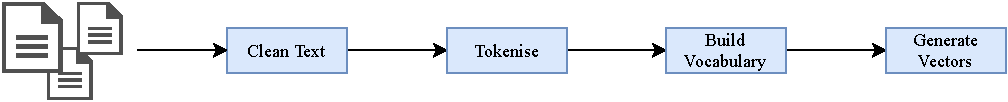
\includegraphics[width=0.8\linewidth]{img/preprocessing_pipeline}
	\caption{Preprocessing pipeline for text}
	\label{fig:preprocessingpipeline}
\end{figure}
The actual steps taken in the preprocessing depends heavily on the use case.

\subsubsection{Clean Text}
\begin{itemize}[noitemsep]
	\item Remove markup
	\item Expand contractions
	\item Truecase
	\item Remove stopwords
	\item Only keep specific word forms
\end{itemize}

\subsubsection{Tokenise}
\begin{itemize}[noitemsep]
	\item Tokenise
	\item Lemmatisation
	\item Stemming\\
	Reduces inflected words to their stem, the root or base forms, even if the stem itself is not a valid word in the language
\end{itemize}

\subsection{Scoring with Jaccard Similarity}
The idea to count the words that are shared between documents to account for similarity stays the same. But the Jaccard Similarity is defined as the size of intersection divided by the size of the union of two sets.

\noindent
\begin{minipage}{0.6\linewidth}
	\begin{equation*}
	J(\text{document}_1,\text{document}_2) = \frac{\text{document}_1\cap\text{document}_2}{\text{document}_1\cup\text{document}_2}
	\end{equation*}
\end{minipage}
\begin{minipage}{0.4\linewidth}
	\begin{center}
		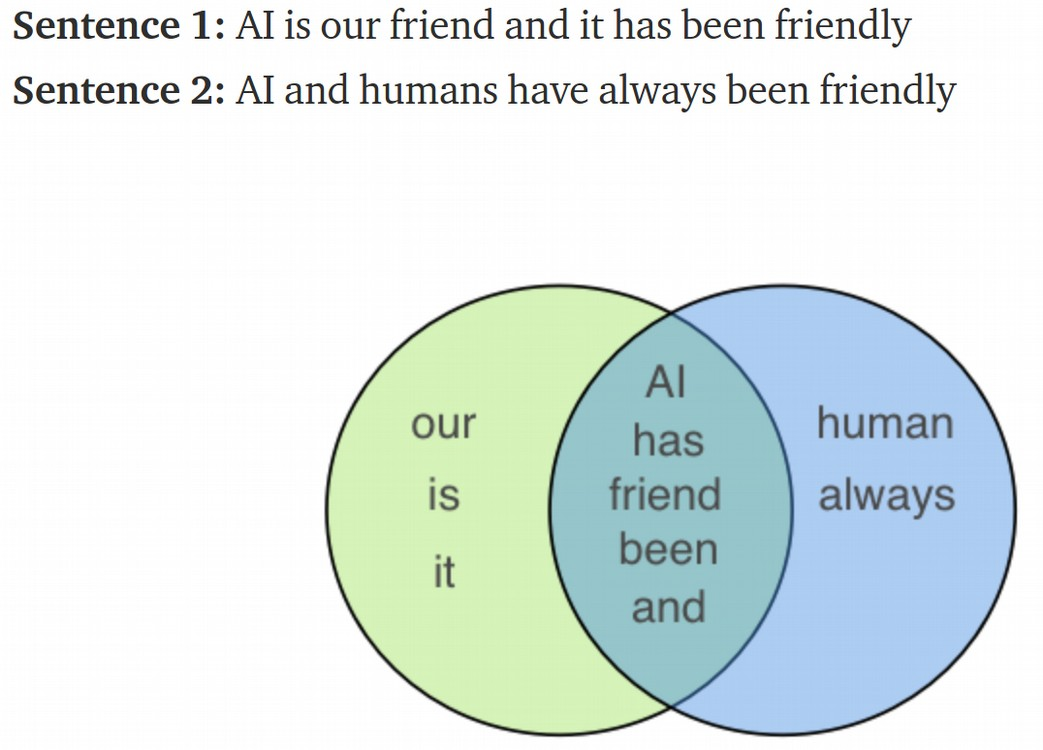
\includegraphics[width=0.9\linewidth]{img/jaccard_set}
	\end{center}
\end{minipage}
Jaccard similarity has the issue of preferring short documents and that it ignores the number a word is occurring.

\subsection{Bag of Words Model}
Focuses on the number of occurrence of words, with the intuition that if a queried word occurs more in the document it is more relevant.
\begin{center}
	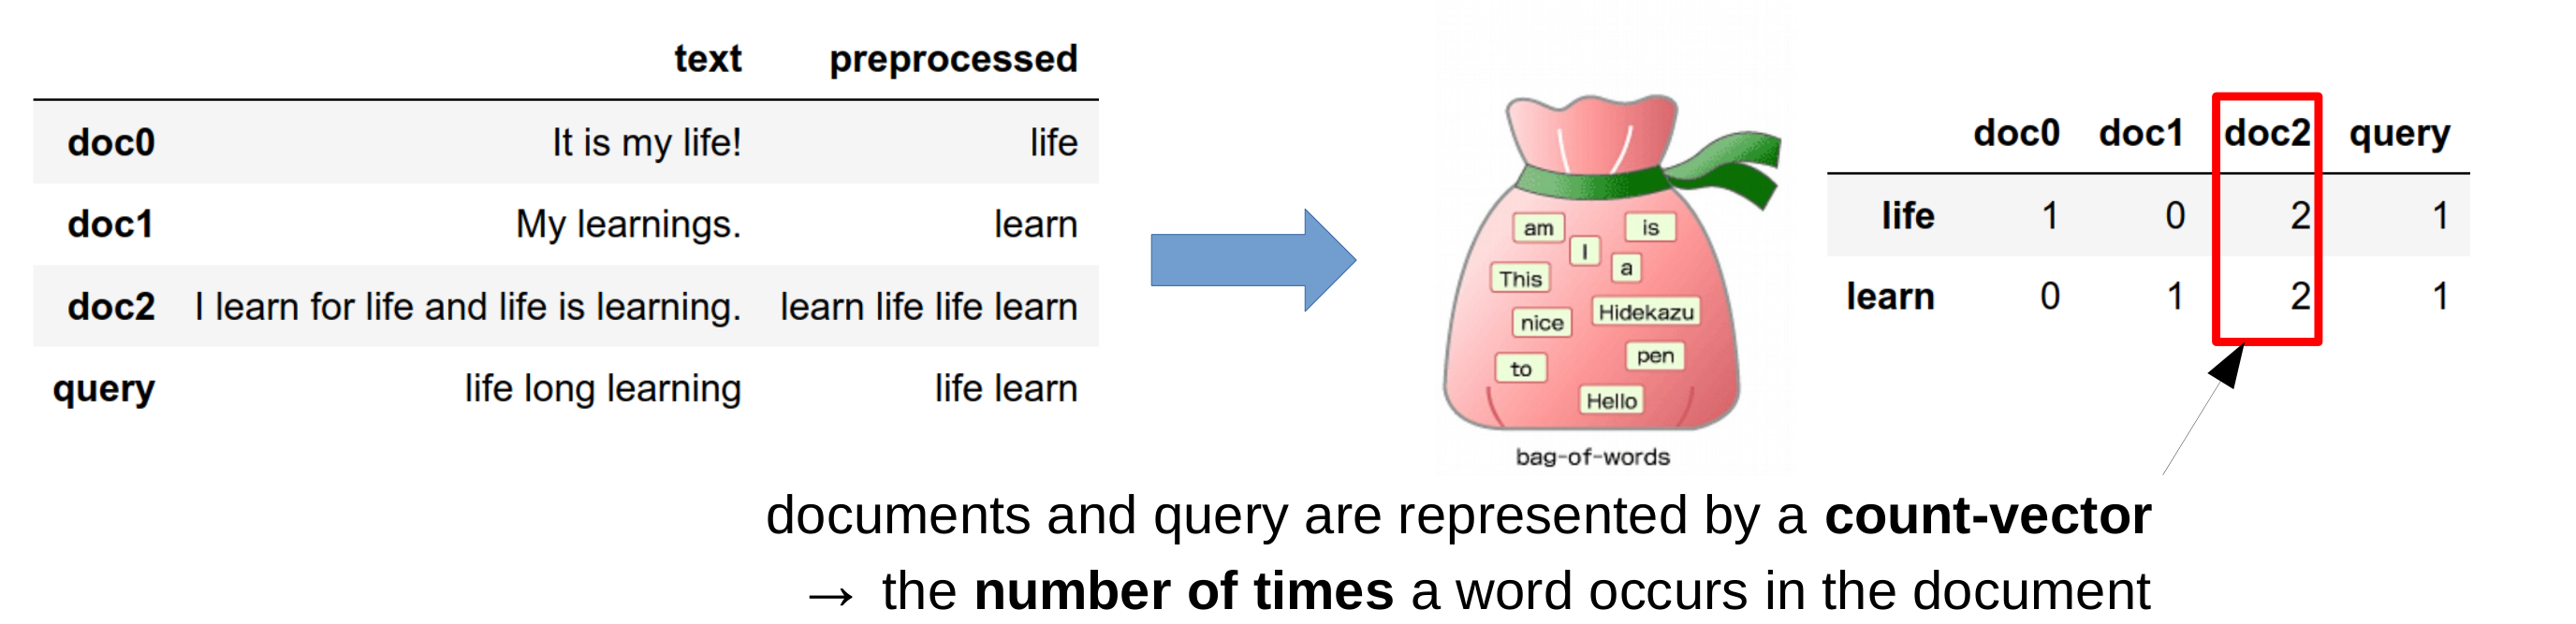
\includegraphics[width=0.8\linewidth]{img/bagofwords_model}
\end{center}
However the Bag of Words model does not consider the ordering of words in a document, and the words must precisely match.

\subsection{Term Frequency Weighting and Transformation}
The raw term frequency is not necessarily the most desirable attribute. A document where a query word occurs more should be handled as more relevant, but a document with 50 occurrences should not be treated 50 times more important than a document with only five occurrences. Thus the relevance should increase sublinear with term frequency
\begin{equation*}
	\text{TF}_{\text{document}} = \underset{\text{word}\in\text{query}\cap\text{document}}{\sum}\log\left( 1 + \text{count}(\text{word},\text{document}) \right)
\end{equation*}
\begin{figure}[H]
	\centering
	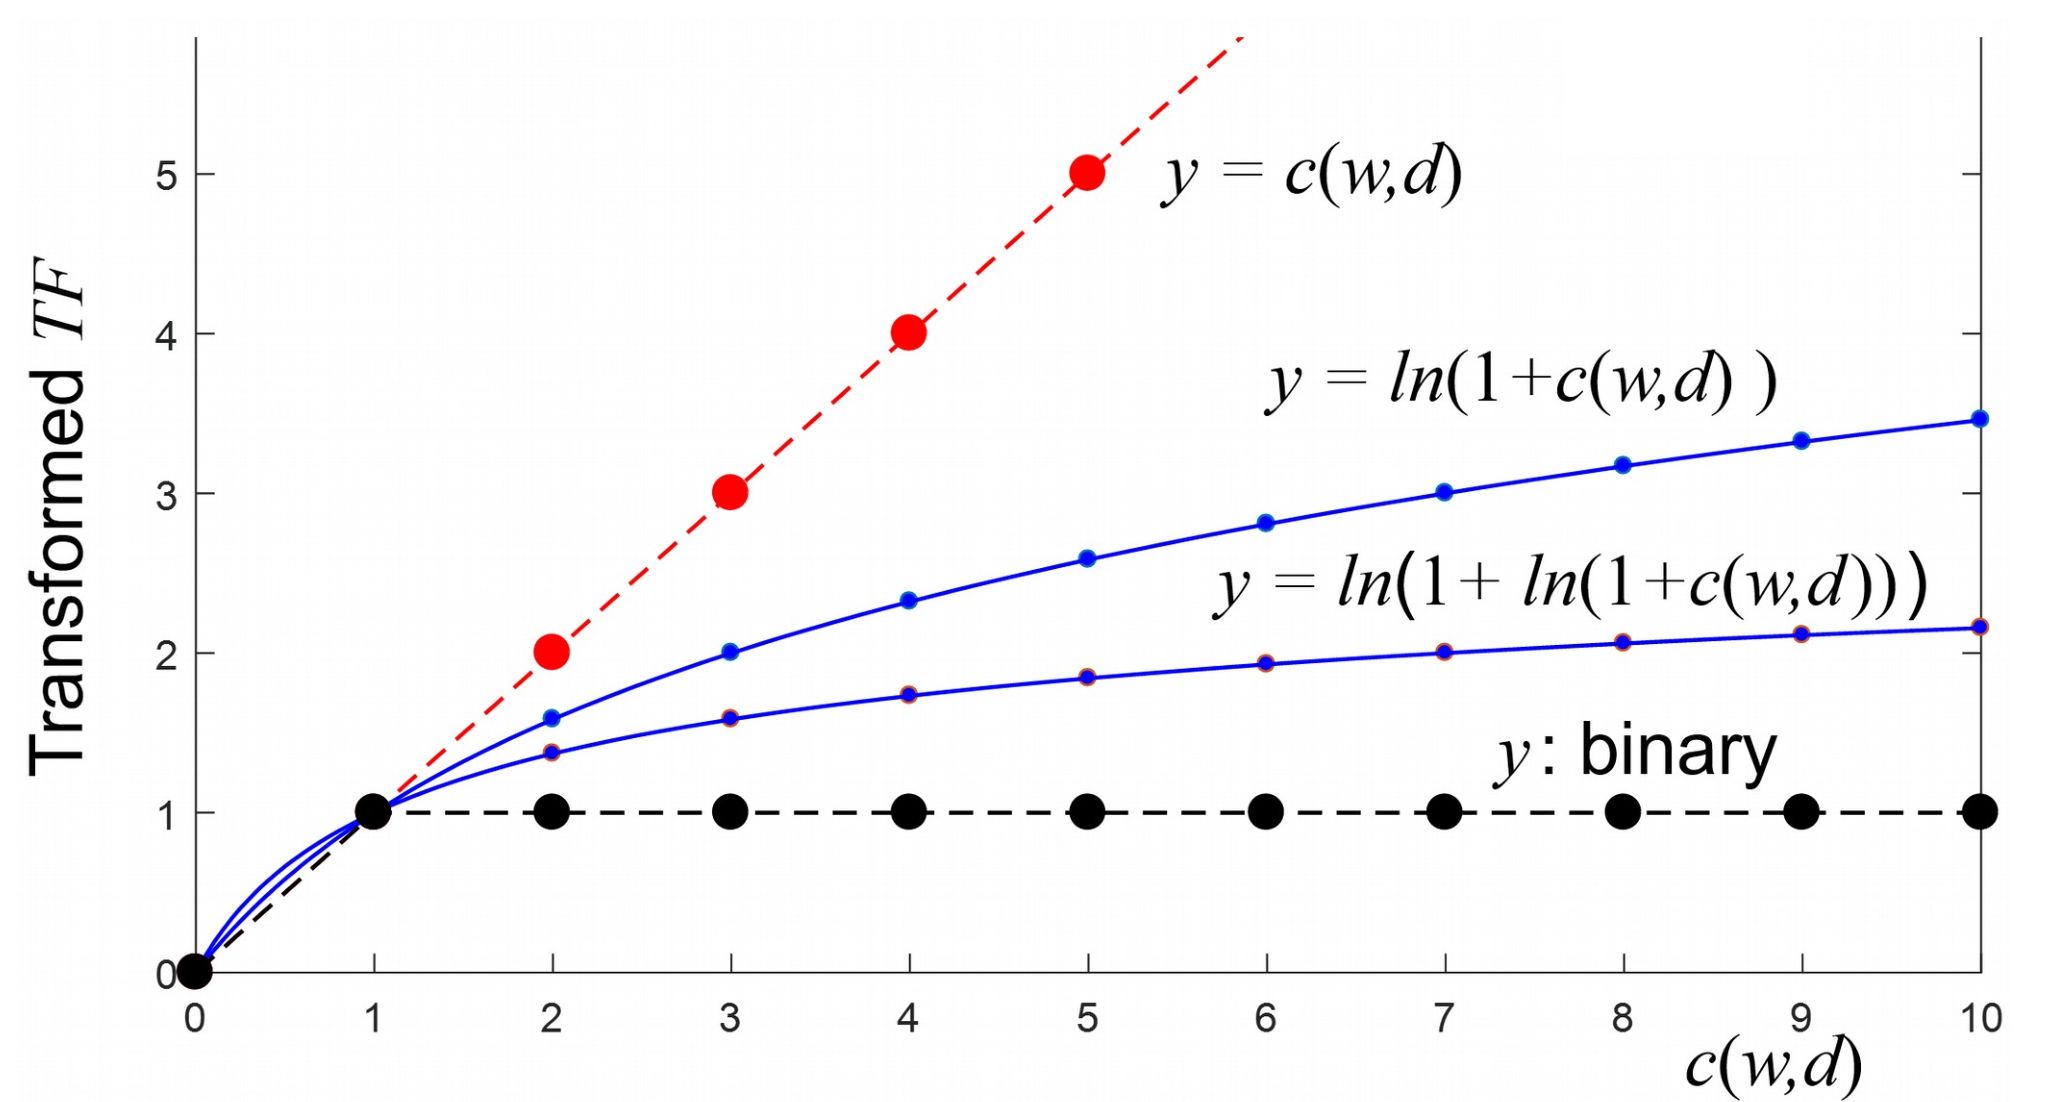
\includegraphics[width=0.6\linewidth]{img/term_frequency_transformation}
	\caption{A sublinear transformation avoids the dominance of single words}
	\label{fig:termfrequencytransformation}
\end{figure}

\subsubsection{(Best Matching) BM25 Term Frequency Transformation}
\begin{equation*}
	y = \frac{(k+1)\cdot c(w,d)}{k+c(w,d)}
\end{equation*}

\subsection{Inverse Document Frequency}
The problem with term frequency lies in the fact that highly frequent words dominate the analysis, but rare and domain specific words may be more informative semantically. Thus positive weights for frequent words but lower weights than for rare words are desirable.
\begin{itemize}[label=]
	\item $\text{DF}_w$: Document Frequency, the number of documents containing word $w$, is the inverse measure of the informativeness of word $w$
	\item $N$: total number of documents in the collection
\end{itemize}
\begin{equation*}
	\text{IDF}_{word}=\log\left(\frac{N}{\text{DF}_{word}}\right)
\end{equation*}
The logarithm is used to dampen the effect of IDF.
\begin{figure}[H]
	\centering
	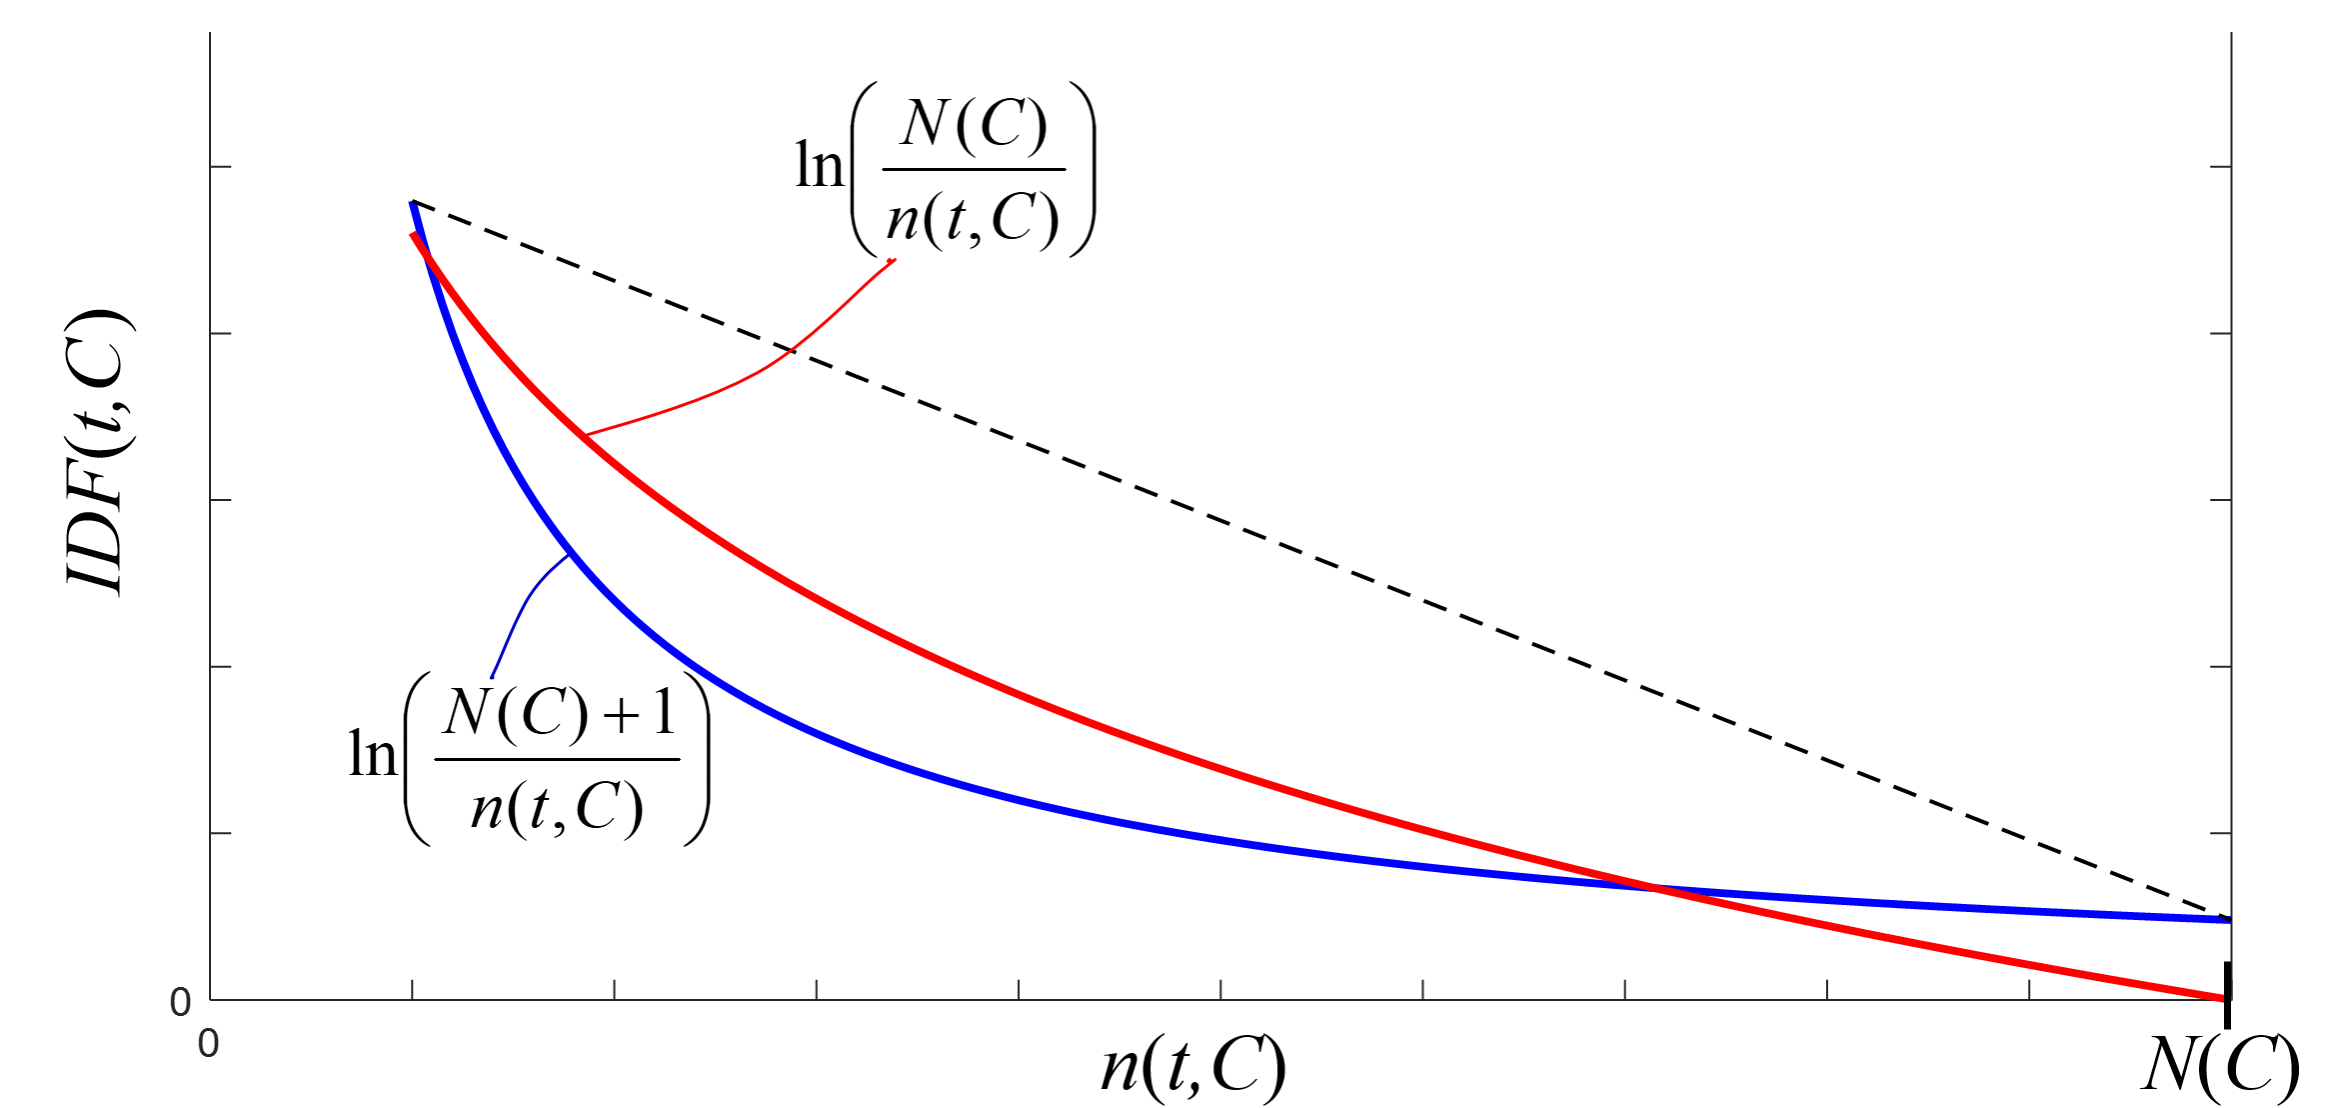
\includegraphics[width=0.6\linewidth]{img/popular_terms_penalty}
	\caption{Popular terms are penalised}
	\label{fig:populartermspenalty}
\end{figure}

\subsection{TF-IDF}
\begin{equation*}
	\text{TF-IDF}_{word} = \text{TF}_{word,doc}\cdot\text{IDF}_{word,coll}
\end{equation*}
Increases with the number of word occurrences within a document and the rarity of the word in the collection. Ranking of documents for a query is done by
\begin{equation*}
	\text{Score}_{query,doc} = \underset{word\in query\cap doc}{\sum} \text{TF-IDF}_{word,doc,coll}
\end{equation*}
\begin{minipage}{\textwidth}
	\renewcommand{\arraystretch}{1.5}
	\begin{tabularx}{\linewidth}{|l|X|p{2cm}|l|X|}
		\cline{1-2}\cline{4-5}
		& TF weights & & & IDF weights\\
		\cline{1-2}\cline{4-5}
		Binary & $ 0 / 1$& & Unary & 1\\
		\cline{1-2}\cline{4-5}
		Counts & $c(t,d)$ & & IDF & $\log\left(\frac{N(C)}{n(t,C)}\right)$\\
		\cline{1-2}\cline{4-5}
		Frequency & $\frac{c(t,d)}{\sum_{\tau\in d} c(\tau,d)}$ & & IDF.
		* & $ 1 + \log\left(\frac{N(C)}{n(t,C)}\right) $ \\
		\cline{1-2}\cline{4-5}
		Log Counts & $ 1 + \log\left( c(t,d) \right) $ & & IDF Smoothed & $\log\left(\frac{N(C)}{1 + n(t,C)}\right)$\\
		\cline{1-2}\cline{4-5}
		\vdots & \vdots & & \vdots & \vdots\\
		\cline{1-2}\cline{4-5}
	\end{tabularx}
\end{minipage}

\subsection{Document Length Normalisation}
Penalise long documents with a document length normaliser, as long documents have a better chance to match any query and are thus less specific. But avoid over-penalisation as documents can be long since they use more words, which should result in more penalisation, or as they have more content, which should be less penalised.
\begin{figure}[H]
	\centering
	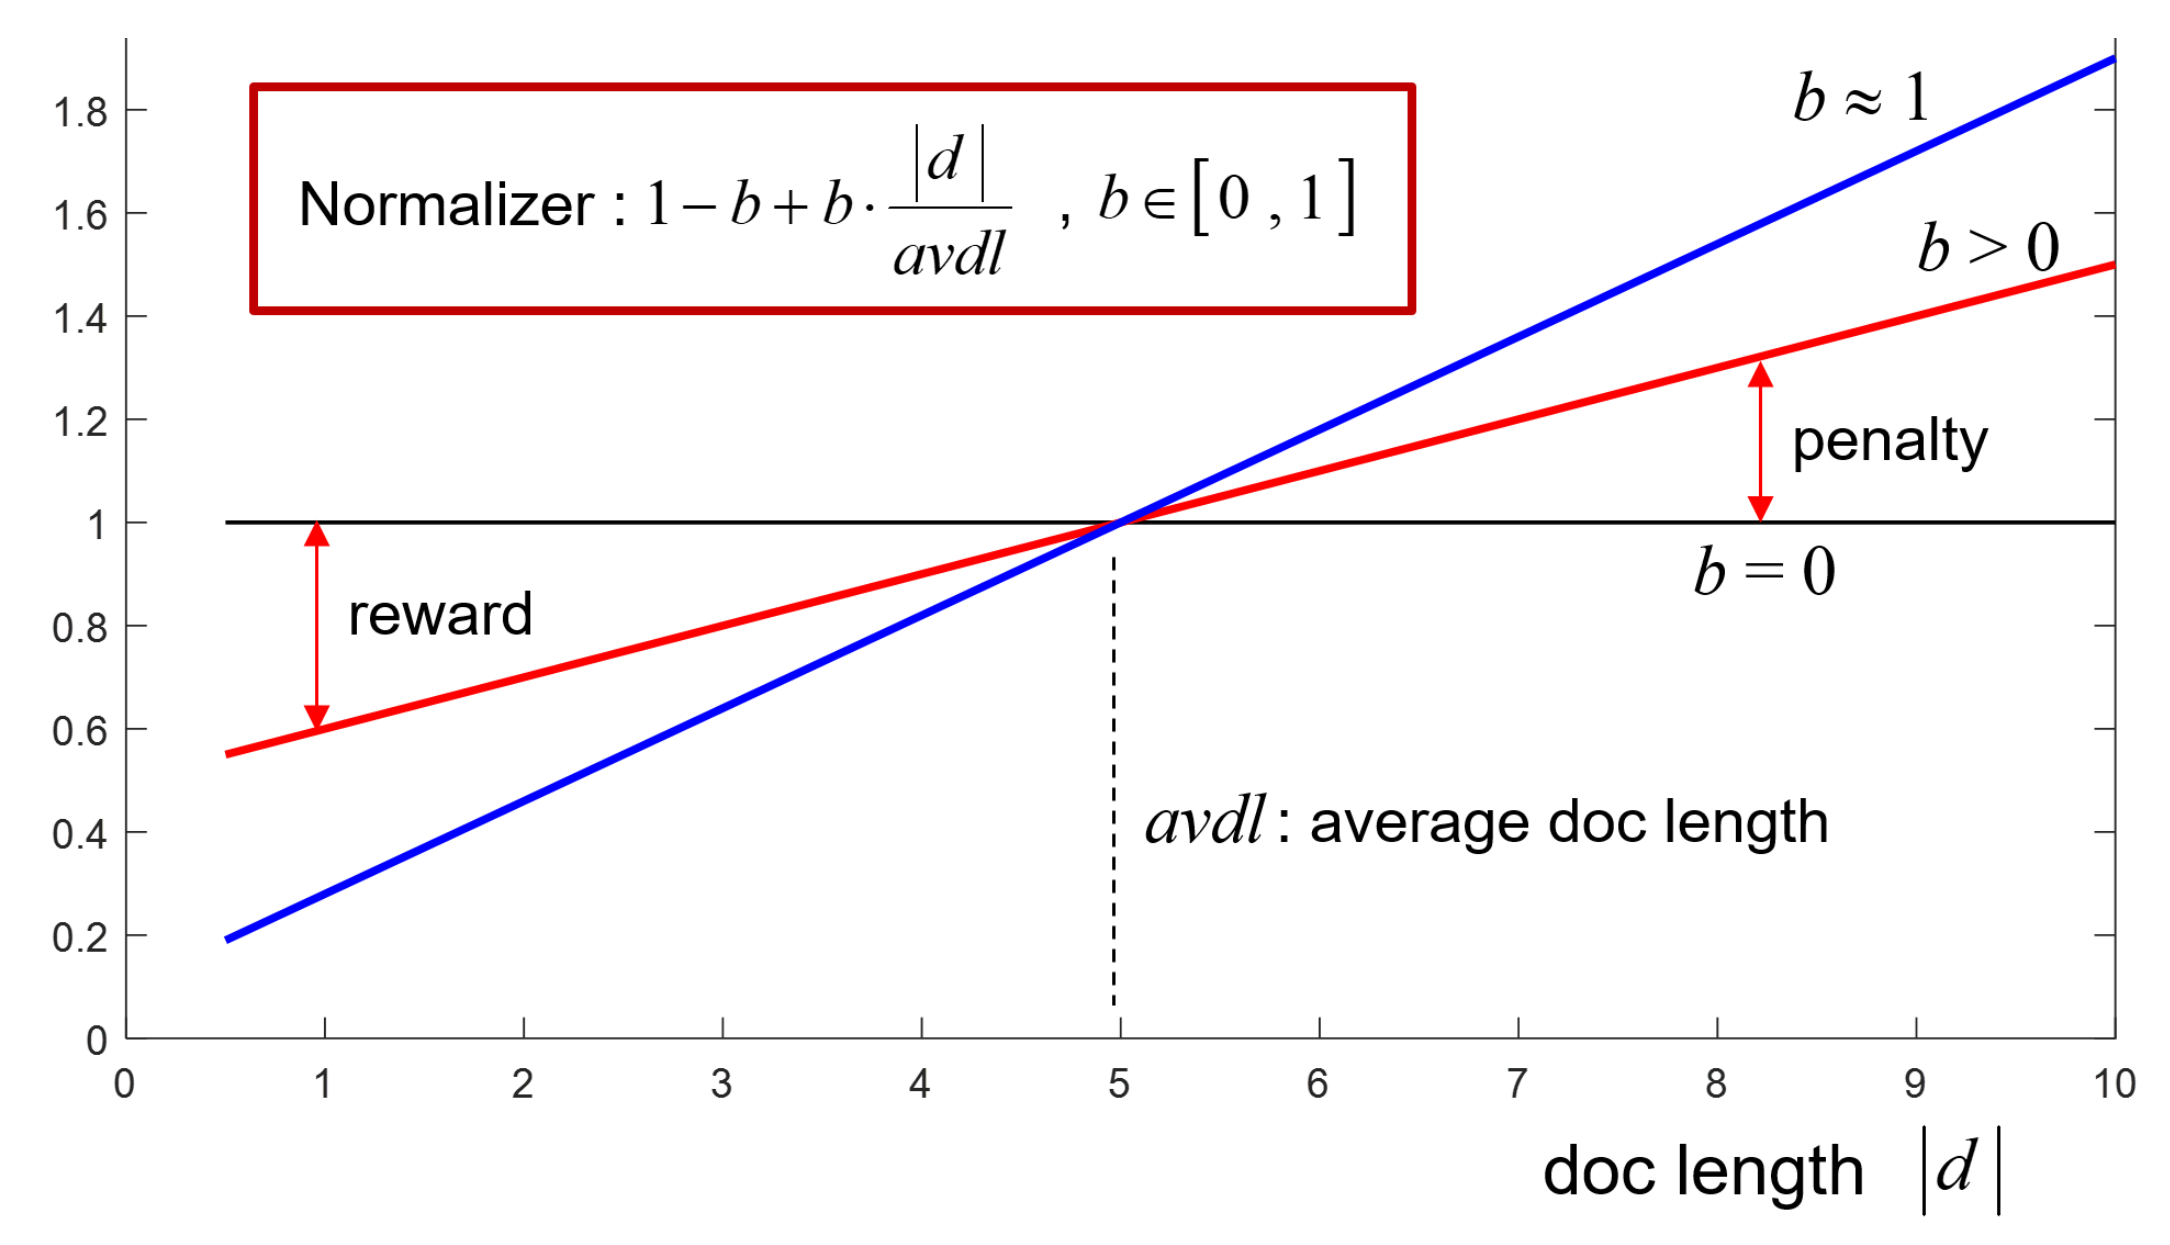
\includegraphics[width=0.6\linewidth]{img/pivot_length_normaliser}
	\caption{Average document length is used as a pivot point}
	\label{fig:pivotlengthnormaliser}
\end{figure}

\subsubsection{State of The Art Okapi BM25+}
Given a Query $Q$ containing keywords $q_1,\dots,q_n$, document $D$'s score is
\begin{equation*}
	\text{score}(D,Q) = \sum_{i=1}^{n}\text{IDF}(q_i) \cdot \left[ \frac{f(q_i,D)\cdot (k_1 + 1)}{f(q_i, D) + k_1\cdot\left( 1 - b + b\cdot\frac{\abs{D}}{\text{avgdl}} \right)} + \delta \right]
\end{equation*}
\begin{equation*}
	\text{IDF}(q_i) = \log \frac{N - n(q_i) + 0.5}{n(q_i) + 0.5}
\end{equation*}
\begin{itemize}[leftmargin=*, labelindent=2cm, labelsep=1cm, noitemsep,nosep]
	\item[$f(q_i,D)$] Term frequency of $q_i$ in document $D$
	\item[$\abs{D}$] length of document $D$
	\item[avgdl] average document length over corpus
	\item[$\delta$] free parameter, default $\delta = 1.0$
	\item[$k_1$] free parameter, $k_1 \in [1.2, 2.0]$
	\item[$b$] free parameter, default $b = 0.75$
	\item[$N$] number of documents in corpus
	\item[$n(q_i)$] number of documents containing $q_i$
\end{itemize}

\subsection{Vector Space Model}
Used to correlate words, sentences and documents by semantic similarity.
\begin{center}
	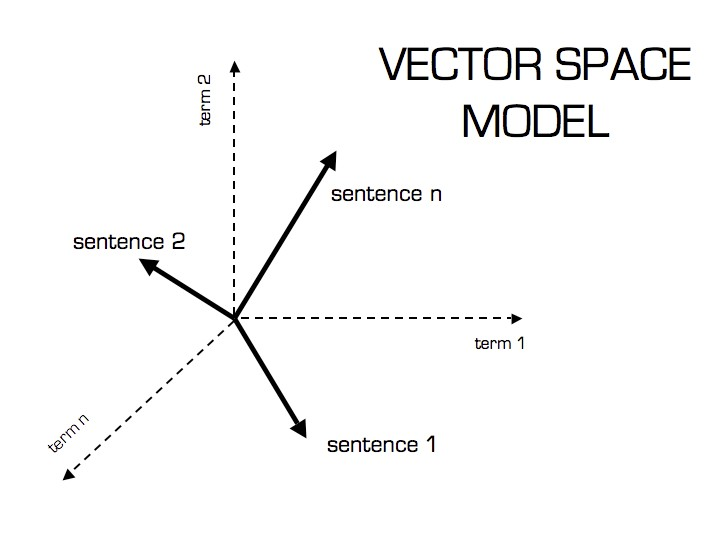
\includegraphics[width=0.5\linewidth]{img/vector_space_model}
\end{center}
For scoring the cosine similarity between documents and a query vector is preferred over the euclidean distance
\begin{itemize}[leftmargin=*, labelindent=3cm, labelsep=1cm, noitemsep]
	\item[similar scores] score vectors are in the same direction, angle between them is almost zero making the cosine lying near one or 100\%
	\item[unrelated scores] score vectors are nearly orthogonal and the cosine is thus near zero
	\item[opposite scores] score vectors in opposite directions, cosine is near minus one or -100\%
\end{itemize}         
The cosine similarity is calculated by
\begin{equation*}
	\cos(d_j,q) = \frac{\bm{d_j}\cdot \bm{q}}{\norm{\bm{d_j}}\norm{\bm{q}}} = \frac{\sum_{i=1}^{N} w_{i,j} w_{i,q} }{\sqrt{\sum_{i=1}^{N}w_{i,j}^2}\sqrt{\sum_{i=1}^{N}w_{i,q}^2}}
\end{equation*}
$\text{L}^2$ norm (Euclidean norm) is the square root of the dot product of the vector $\bm{p}$ with itself, and scales a vector to its unit-length
\begin{equation*}
	\norm{\bm{p}} = \sqrt{p_1^2 + p_2^2 + \dots + p_n^2} = \sqrt{\bm{p}\cdot\bm{p}}
\end{equation*}
Normalising all vectors to unit vectors this way allows for the dot-product to measure similarity, and do it in a more efficient way than cosine similarity. The dot product between two vectors $\bm{d_j}$ and $\bm{q}$ is high if $w_{ij}$ and $w_{iq}$ have similar characteristics, and is equivalent to the cosine similarity if the vectors are normalised.







\end{document}
